\documentclass[10pt,twocolumn]{article}
\raggedbottom

\usepackage[margin=1in]{geometry}
\usepackage{amsmath,amssymb}
\usepackage{booktabs}
\usepackage{hyperref}
\usepackage{listings}
\usepackage{xcolor}
\usepackage{enumitem}
\usepackage{microtype}
\usepackage{caption}
\captionsetup{font=small,labelfont=bf}
\usepackage{abstract}
\usepackage{tikz}
\usepackage{needspace}
\usepackage{placeins}
\usepackage{float}
\usepackage{etoolbox}
\usetikzlibrary{arrows.meta,positioning,calc,fit,backgrounds}

\setlength{\absleftindent}{0.5in}
\setlength{\absrightindent}{0.5in}
\renewcommand{\abstractnamefont}{\normalfont\bfseries\small}
\renewcommand{\abstracttextfont}{\normalfont\small}
\setcounter{topnumber}{4}
\setcounter{bottomnumber}{2}
\setcounter{totalnumber}{6}
\renewcommand{\topfraction}{0.95}
\renewcommand{\bottomfraction}{0.9}
\renewcommand{\textfraction}{0.05}
\renewcommand{\floatpagefraction}{0.8}
\setlength{\textfloatsep}{8pt plus 2pt minus 2pt}
\setlength{\floatsep}{6pt plus 2pt minus 2pt}
\setlength{\intextsep}{6pt plus 2pt minus 2pt}

\hypersetup{colorlinks=true,linkcolor=blue!60!black,urlcolor=blue!60!black}

\lstdefinestyle{code}{
    basicstyle=\ttfamily\footnotesize,
    keywordstyle=\bfseries\color{blue!70!black},
    commentstyle=\color{green!40!black},
    showstringspaces=false,
    columns=flexible,
    breaklines=true,
    frame=single,
    framerule=0.4pt,
    rulecolor=\color{gray!50},
    backgroundcolor=\color{gray!5},
    xleftmargin=2pt,
    xrightmargin=2pt,
    aboveskip=4pt,
    belowskip=4pt,
}
% Keep headings with a few lines of following text, without forcing large gaps.
\preto{\section}{\needspace{10\baselineskip}}
\preto{\subsection}{\needspace{6\baselineskip}}
% Keep short code blocks together when possible; allow long ones to break.
\AtBeginEnvironment{lstlisting}{\needspace{8\baselineskip}}

\title{Base: A Board-Level Software ISA\\with Build-Time Dependent Type Checking}
\author{\url{https://github.com/unnamedlambda/base}}
\date{}

\begin{document}

\twocolumn[
\begin{@twocolumnfalse}
\maketitle
\vspace{-1em}
\begin{onecolabstract}
A modern system board often contains many hardware units, each with its own
ISA: a CPU, a GPU, and specialized accelerators. Programming them correctly
requires reasoning about value-dependent properties such as memory layouts,
buffer offsets, and cross-device data flow. Dependent type theory can express these
constraints, but languages with sufficiently expressive type systems often
incur managed run-time overhead (for example, garbage collection,
reference-count traffic, boxing, and other run-time support costs). We therefore
want dependent type checking to happen at build time and to execute code
that maps well onto modern hardware, as modern systems languages commonly
do (e.g., C and C++).

Base solves this with a clean separation. At build time, Lean~4~\cite{lean4}
with dependent types produces a serializable execution artifact containing
Cranelift~\cite{cranelift} IR text, an initial memory layout, and one or
more compiled-function entry points. At run time, a Rust engine JIT-compiles
the IR and calls the selected entry point. No type checker, no interpreter,
no garbage collector runs at run time---just compiled machine code calling
hardware through FFI primitives. The data artifact is the only thing that
crosses from the verified world to the executable world, and it contains no
closures, callbacks, or run-time artifacts from Lean.

This supports a modern heterogeneous system with multiple ISAs following
different conventions. The ISAs do not need to be designed to work intuitively
together---they can be awkward, optimized purely for silicon, because the
dependent type system absorbs their complexity at build time. Base is
evaluated on CPU, GPU, and heterogeneous workloads. On the evaluated
workloads, it is competitive with idiomatic Rust and native GPU frameworks.
\end{onecolabstract}
\vspace{1em}
\end{@twocolumnfalse}
]

% ===================================================================
\section{Introduction}
\label{sec:intro}

Board-level software must coordinate multiple ISAs on one system board
(CPU, GPU, tensor/crypto engines, and other accelerators). Doing this
correctly requires reasoning about shared memory layouts,
buffer offsets, dispatch ordering, and data flow between devices.

These are value-dependent invariants. A buffer offset must be less than the
memory size. A GPU dispatch must happen after initialization. A data layout
must be consistent between the CPU view and the GPU view. Dependent types
allow types to depend on values, so bounds, layout relationships, and
sequencing conditions can participate directly in artifact construction and
checking. That is useful here because offsets, sizes, and dispatch structure
all depend on concrete build-time values.

Dependent type checking requires substantial compile-time machinery.
In Lean~4, checking depends on term reduction/normalization. None of this
proof-assistant machinery should be in the run-time path.

Base separates the problem in two:

\begin{enumerate}[nosep,leftmargin=*]
\item \textbf{Build time} (Lean~4): Verify program structure with dependent
  types. Output a serializable data artifact containing Cranelift IR text,
  an initial memory layout, and named entry points into the generated CLIF,
  with no Lean run-time artifacts.
\item \textbf{Run time} (Rust engine): JIT-compile the IR via Cranelift.
  Execute selected CLIF functions against shared memory, calling hardware through typed FFI
  primitives.
\end{enumerate}

The data artifact is inert: bytes, offsets, IR text, integer tags. It is the
only value that crosses from the verified world to the executable world.

A consequence: ISAs targeted by this system do not need to be programmer-friendly.
If the specification language handles complexity, hardware can be optimized
purely for silicon efficiency---what might be called \emph{awkward ISAs}.
Because no human or general-purpose compiler targets the IR directly,
instruction sets can be irregular---non-power-of-two register files,
application-specific operations, unusual word sizes---and the Lean
specification provides verified transformations to each device on the bus.

% ===================================================================
\section{Architecture}
\label{sec:arch}

Figure~\ref{fig:arch} shows the system. Lean constructs the data artifact
at build time; the Rust engine consumes it at run time.

\begin{figure}[H]
\centering
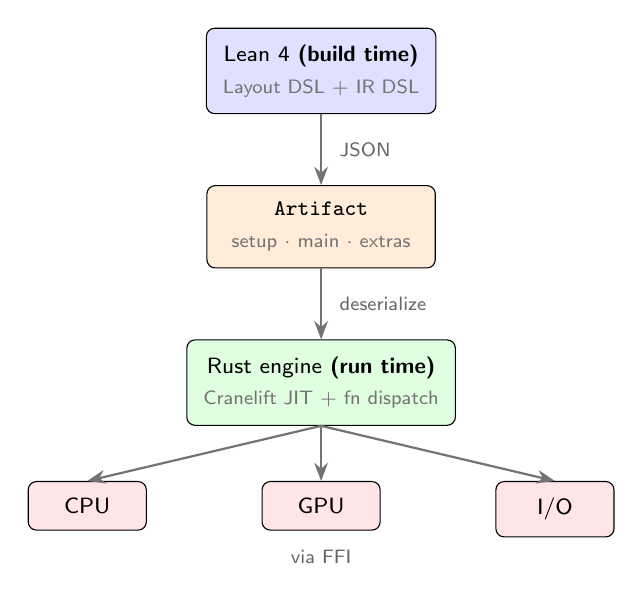
\begin{tikzpicture}[
    >=Stealth,
    box/.style={draw, rounded corners=3pt,
                font=\footnotesize\sffamily, fill=#1, text=black,
                inner sep=6pt, align=center},
    box/.default=gray!8,
    lbl/.style={font=\scriptsize\sffamily, text=black!60},
    arr/.style={->, thick, color=black!55},
  ]
  % Build time — Lean
  \node[box=blue!12, minimum width=2.9cm] (lean)
    {Lean~4 \textbf{(build time)}\\[2pt]
     {\scriptsize\sffamily\color{black!55} Layout DSL $+$ IR DSL}};

  % The data artifact
  \node[box=orange!15, minimum width=2.9cm, below=0.9 of lean] (artifact)
    {\texttt{Artifact}\\[2pt]
     {\scriptsize\sffamily\color{black!55} setup $\cdot$ main $\cdot$ extras}};
  \draw[arr] (lean) -- node[lbl, right=3pt] {JSON} (artifact);

  % Run time — Rust engine
  \node[box=green!12, minimum width=2.9cm, below=0.9 of artifact] (engine)
    {Rust engine \textbf{(run time)}\\[2pt]
     {\scriptsize\sffamily\color{black!55} Cranelift JIT $+$ fn dispatch}};
  \draw[arr] (artifact) -- node[lbl, right=3pt] {deserialize} (engine);

  % Hardware targets
  \node[box=red!10, minimum width=1.5cm, below left=0.7 and 0.5 of engine] (cpu) {CPU};
  \node[box=red!10, minimum width=1.5cm, below=0.7 of engine]             (gpu) {GPU};
  \node[box=red!10, minimum width=1.5cm, below right=0.7 and 0.5 of engine] (net) {I/O};
  \draw[arr] (engine.south) -- (cpu.north);
  \draw[arr] (engine.south) -- (gpu.north);
  \draw[arr] (engine.south) -- (net.north);
  \node[lbl, below=0.12 of gpu.south, anchor=north] {via FFI};
\end{tikzpicture}
\caption{Lean builds the data artifact at build time; the Rust engine
consumes it at run time and dispatches via FFI.}
\label{fig:arch}
\end{figure}

The build-time phase runs once per program revision. Lean~4 type-checks
the specification, emits a flat memory layout and Cranelift IR text,
and serializes the resulting \texttt{Artifact} as JSON.
Rust \texttt{build.rs} then validates that JSON against the Rust data types,
re-serializes it to bincode, and embeds it in the executable via
\texttt{include\_bytes!}. At run time the engine deserializes the embedded
artifact, JIT-compiles the IR once during \texttt{Base::new}, and executes
the \texttt{main} algorithm or a named algorithm from \texttt{extras} by
calling its compiled function index.

% ===================================================================
\section{The Data Artifact}
\label{sec:artifact}

A Base program is a single \texttt{Artifact}, serialized as JSON:

\begin{lstlisting}[style=code,
  morekeywords={pub,struct,Vec,String,usize,u8,u32,HashMap}]
pub struct Artifact {
  pub setup: Setup,
  pub main: Algorithm,
  pub extras: HashMap<String, Algorithm>,
}
pub struct Setup {
  pub cranelift_ir: String,
  pub memory_size: usize,
  pub io_offsets: IoOffsets,
  pub initial_memory: Vec<u8>,
}
pub struct IoOffsets {
  pub data_ptr: usize,
  pub data_len: usize,
  pub out_ptr: usize,
  pub out_len: usize,
}
pub struct Algorithm {
  pub fn_idx: u32,
  pub output: Vec<OutputBatchSchema>,
}
\end{lstlisting}

\texttt{Setup} contains the module-level Cranelift IR text, memory size,
runtime input/output slots, and byte-level initial memory generated by
Lean. \texttt{Algorithm} is an entry point into that compiled module:
\texttt{fn\_idx} selects one JIT-compiled function, and \texttt{output}
describes optional Arrow record batches to read from shared memory after
the call. A single-artifact program uses \texttt{main}; multi-stage flows
put additional entry points in \texttt{extras}, so all stages share one
memory image and one Cranelift compilation.

Orchestration is represented either inside generated CLIF
functions or by explicit calls to different \texttt{Algorithm} entry points
by the host application.

\subsection{Shared Memory}

All state lives in a single pinned byte array. When a \texttt{Base}
struct is created, the array is initialized from \texttt{initial\_memory},
which holds program data, string constants, and scratch buffers produced
by Lean. Every JIT-compiled function receives one argument: a pointer to
byte~0 of this array.

For caller-provided input and output buffers, \texttt{Setup.io\_offsets}
specifies where the engine writes transient pointer slots before each
\texttt{execute()} call (Table~\ref{tab:iooffsets}). These offsets are
part of the artifact rather than a hard-coded Rust header.

\begin{table}[H]
\centering\small
\caption{Runtime input/output slots specified by \texttt{IoOffsets}.}
\label{tab:iooffsets}
\begin{tabular}{@{}ll@{}}
\toprule
\textbf{Field} & \textbf{Value written before execution} \\
\midrule
\texttt{data\_ptr} & pointer to caller input bytes \\
\texttt{data\_len} & caller input length \\
\texttt{out\_ptr}  & pointer to caller output buffer \\
\texttt{out\_len}  & caller output length \\
\bottomrule
\end{tabular}
\end{table}

CLIF code reads \texttt{data\_ptr}/\texttt{data\_len} to access caller
input and \texttt{out\_ptr}/\texttt{out\_len} to write results---zero
copies. GPU, CUDA, hash-table, network, and database contexts are managed
through FFI calls that initialize and pass context handles explicitly, not
through a single serialized context offset in the artifact.

\needspace{14\baselineskip}
\subsection{Execution}

\begin{lstlisting}[style=code,
  morekeywords={let,mut,fn,pub}]
// One-shot
let artifact = Artifact::from_bytes(ARTIFACT_BINARY);
let results = run(artifact.setup, artifact.main)?;

// Compile once, execute many
let artifact = Artifact::from_bytes(ARTIFACT_BINARY);
let mut base = Base::new(artifact.setup)?;
base.execute(&artifact.main, &data)?;

// Named multi-stage entry points
let prep = &artifact.extras["prep"];
let infer = &artifact.extras["infer"];
base.execute(prep, &input)?;

// Zero-copy output
base.execute_into(infer, &in, &mut out)?;
\end{lstlisting}

After JIT compilation, \texttt{execute()} is a hot path: callers pass
data by reference, the engine writes the caller pointers to the configured
\texttt{IoOffsets}, and then calls \texttt{algorithm.fn\_idx} in the
compiled module. CLIF code reads caller data directly.

\subsection{FFI: From Rust to C~ABI to Cranelift}
\label{sec:ffi}

Hardware access follows a three-step chain. First, a Rust function wraps
a driver library (wgpu~\cite{wgpu}, CUDA, LMDB~\cite{lmdb}, TCP) behind
\texttt{extern "C"} linkage:

\begin{lstlisting}[style=code,
  morekeywords={unsafe,extern,fn,let,mut,match}]
unsafe extern "C" fn cl_file_read_to_ptr(
    path_ptr: *const u8, // filename pointer
    dst_ptr: *mut u8,    // destination pointer
    file_offset: i64,    // seek position
    size: i64,           // bytes to read
) -> i64 {
    let filename = read_cstr_ptr(path_ptr);
    let mut file = match fs::File::open(&filename) {
        Ok(f) => f,  Err(_) => return -1,
    };
    // ... read into dst_ptr, return count
}
\end{lstlisting}

Second, the engine registers this function pointer with the Cranelift JIT
builder under its symbol name:

\begin{lstlisting}[style=code,
  morekeywords={builder}]
builder.symbol("cl_file_read_to_ptr",
    cl_file_read_to_ptr as *const u8);
\end{lstlisting}

Third, Lean can target the same symbol in two equivalent ways. Small
benchmarks in this repository often emit the raw CLIF directly:

\begin{lstlisting}[style=code]
sig0 = (i64, i64, i64, i64) -> i64 system_v
fn0 = %cl_file_read_to_ptr sig0

block4:
    v3 = iconst.i64 256
    v4 = iadd v0, v3      ; filename pointer
    v5 = iconst.i64 8192
    v6 = iadd v0, v5      ; destination pointer
    v7 = iconst.i64 0
    v8 = iconst.i64 4096
    v9 = call fn0(v4, v6, v7, v8)
\end{lstlisting}

Larger applications use the IR builder, which produces the same external
declaration while returning a typed handle:

\begin{lstlisting}[style=code]
def declareFileRead : IRBuilder FnRef :=
  declareFFI "cl_file_read_to_ptr"
    [.i64, .i64, .i64, .i64] (some .i64)
\end{lstlisting}

In both cases the generated \texttt{cranelift\_ir} contains the same
external symbol reference. At JIT time, Cranelift resolves
\texttt{\%cl\_file\_read\_to\_ptr} to the registered pointer---a direct native
call, no extra dispatch layer. The same three-step pattern applies to
all registered FFI symbols (Table~\ref{tab:ffi}).

\begin{table}[H]
\centering\small
\caption{FFI primitive categories (88 registered symbols total).}
\label{tab:ffi}
\begin{tabular}{@{}lrp{0.42\columnwidth}@{}}
\toprule
\textbf{Category} & \textbf{n} & \textbf{Examples} \\
\midrule
Hash table  & 8  & init, insert, lookup, increment \\
GPU (wgpu)  & 9  & init, ptr upload, dispatch \\
CUDA/cuBLAS & 39 & streams, graphs, PTX launch, GEMM \\
File/math/I/O & 9 & file read/write, trig, stdin/stdout \\
Networking  & 8  & listen, connect, send \\
Database    & 10 & LMDB transactions \\
Threading   & 5  & spawn, join, direct call \\
\bottomrule
\end{tabular}
\end{table}

Adding a new device means: (1)~write \texttt{extern "C"} Rust wrappers,
(2)~register symbols in the JIT builder, (3)~add a
\texttt{declareFFI} bundle in Lean. The artifact format and function-index
dispatch model do not change.

% ===================================================================
\section{Specification in Lean}
\label{sec:lean}

The goal of the Lean build-time phase is always the same: produce a valid
\texttt{Artifact}. Figure~\ref{fig:pipeline}
shows the end-to-end picture. What Lean emits---Cranelift IR text, an
initial memory layout, and \texttt{main}/\texttt{extras} entry points---is
fixed by that type. Any
Lean code that type-checks and produces such an artifact is a legitimate front
end. The DSLs described below are one convenient approach used in this
repository, built from standard functional programming techniques in Lean;
they are not the only option, and users may write whatever transformations
suit their domain.

\begin{figure}[H]
\centering
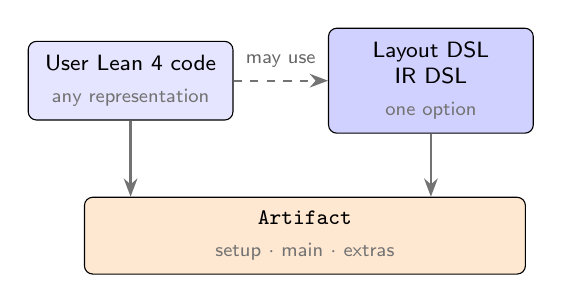
\begin{tikzpicture}[
    >=Stealth,
    box/.style={draw, rounded corners=3pt, font=\footnotesize\sffamily,
                fill=#1, inner sep=5pt, align=center},
    box/.default=gray!8,
    lbl/.style={font=\scriptsize\sffamily, color=black!60},
    arr/.style={->, thick, color=black!55},
  ]
  % User's Lean code — free-form
  \node[box=blue!10, minimum width=2.6cm] (src)
    {User Lean~4 code\\[2pt]
     {\scriptsize\color{black!55} any representation}};

  % DSLs (optional path)
  \node[box=blue!18, minimum width=2.6cm, right=1.2 of src] (dsl)
    {Layout DSL\\IR DSL\\[2pt]
     {\scriptsize\color{black!55} one option}};

  % Data artifact (fixed output)
  \node[box=orange!18, minimum width=5.6cm, below=0.8 of dsl,
        xshift=-1.6cm] (artifact)
    {\texttt{Artifact}\\[2pt]
     {\scriptsize\color{black!55}
      setup $\cdot$ main $\cdot$ extras}};

  \draw[arr] (src.south) -- (artifact.north -| src.south);
  \draw[arr, dashed] (src) -- node[lbl, above=1pt] {may use} (dsl);
  \draw[arr] (dsl.south) -- (artifact.north -| dsl.south);
\end{tikzpicture}
\caption{Any Lean code that produces the data artifact is valid. In this
repository, both raw CLIF string emitters and the monadic DSL are used;
both are just front ends to the same artifact.}
\label{fig:pipeline}
\end{figure}

\subsection{The Transformation}

Figure~\ref{fig:transform} shows what the DSLs do at a high level.
On the left: typed Lean values---field declarations with their sizes
and alignments, and SSA operations with their operands. On the right:
the two outputs that populate the data artifact. The transformation is
purely functional; standard stateful-computation patterns in Lean
thread a byte cursor through field declarations and an instruction
list through IR construction. The key property is that Lean computes
offsets, sizes, and SSA value IDs during artifact construction, which
lets the surrounding types and builders impose constraints before any
code runs.

\begin{figure}[H]
\centering
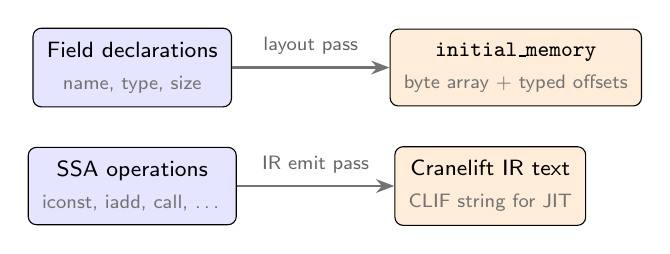
\begin{tikzpicture}[
    >=Stealth,
    box/.style={draw, rounded corners=3pt, font=\footnotesize\sffamily,
                fill=#1, inner sep=5pt, align=center, minimum width=2.4cm},
    box/.default=gray!8,
    lbl/.style={font=\scriptsize\sffamily, color=black!60},
    arr/.style={->, thick, color=black!55},
  ]
  % Inputs
  \node[box=blue!10] (fld)
    {Field declarations\\[2pt]{\scriptsize\color{black!55}name, type, size}};
  \node[box=blue!10, below=0.5 of fld] (ops)
    {SSA operations\\[2pt]{\scriptsize\color{black!55}iconst, iadd, call, \ldots}};

  % Outputs
  \node[box=orange!15, right=2.0 of fld] (mem)
    {\texttt{initial\_memory}\\[2pt]{\scriptsize\color{black!55}byte array + typed offsets}};
  \node[box=orange!15, right=2.0 of ops] (ir)
    {Cranelift IR text\\[2pt]{\scriptsize\color{black!55}CLIF string for JIT}};

  \draw[arr] (fld) -- node[lbl, above=1pt] {layout pass} (mem);
  \draw[arr] (ops) -- node[lbl, above=1pt] {IR emit pass} (ir);
\end{tikzpicture}
\caption{The two DSL passes: field declarations map to a typed byte layout;
SSA operations map to Cranelift IR text. Both are pure Lean functions.}
\label{fig:transform}
\end{figure}

\subsection{Memory Layout}

The layout stage produces the concrete \texttt{initial\_memory} byte
array, the total \texttt{memory\_size}, and typed references to
important regions. In the current applications those outputs include
string constants, headers, descriptors, scratch buffers, and
runtime-visible input/output regions.

What matters is that later CLIF generation refers to these generated
locations by named Lean values rather than manually duplicated offsets.
Lean computes the byte positions and serialized initial contents at
build time, so the artifact carries both a concrete memory image and
the locations that the generated code will read, write, and pass to
FFI calls.

% ===================================================================
\section{Example: GPU Path Tracer}
\label{sec:example}

To illustrate the full pipeline, this section traces a complete application: a
$4096 \times 4096$ Cornell box path tracer with 5-bounce ray tracing.
The entire specification---WGSL shader, Cranelift IR, BMP header, and
memory layout---is a single Lean file.

\subsection{What Lean Produces}

The Lean file constructs the full \texttt{Artifact}:

\paragraph{Memory layout.} The \texttt{initial\_memory} byte array
contains, at known offsets: the output filename string, a 54-byte BMP
header (with width, height, and pixel format pre-filled), the WGSL
shader source (${\sim}$16\,KB of text), a GPU binding descriptor, and a
zero-filled pixel buffer large enough for $4096 \times 4096 \times 4$
bytes (${\sim}$67\,MB). Every offset is a named Lean constant, checked
against the total \texttt{memory\_size}.

\paragraph{Cranelift IR.} The IR builder emits a single function
(\texttt{u0:0}) that orchestrates the GPU through seven FFI calls:

\begin{lstlisting}[style=code]
def clifIrSource : String := buildProgram do
  let gpu <- declareGpuFFI
  let fnWr <- declareFileWrite
  let ptr <- entryBlock
  -- GPU lifecycle: init, buffer, shader,
  -- dispatch, download, cleanup
  callVoid gpu.fnInit [ptr]
  let sz <- iconst64 pixelBytes
  let buf <- call gpu.fnCreateBuffer [ptr, sz]
  let pipe <- call gpu.fnCreatePipeline
    [ptr, shaderOff, bindOff, one32]
  let _ <- call gpu.fnDispatch
    [ptr, pipe, wgX, wgY, one32]
  let _ <- call gpu.fnDownload
    [ptr, buf, pixelOff, sz]
  callVoid gpu.fnCleanup [ptr]
  -- Write BMP: header (54B) + pixels
  let total <- iconst64 (54 + pixelBytes)
  let _ <- writeFile0 ptr fnWr
    filenameOff headerOff total
  ret
\end{lstlisting}

\needspace{8\baselineskip}
\paragraph{Algorithm entry point.} The artifact's \texttt{main}
algorithm selects that function:

\begin{lstlisting}[style=code]
def raytraceAlgorithm : Algorithm := {
  fn_idx := IR.mainFnIdx
  output := []
}
\end{lstlisting}

\subsection{What the Engine Does}

Figure~\ref{fig:raytrace} shows the run-time execution flow. The Rust
side is three lines: deserialize, construct \texttt{Base}, call
\texttt{execute}.

\begin{figure}[H]
\centering
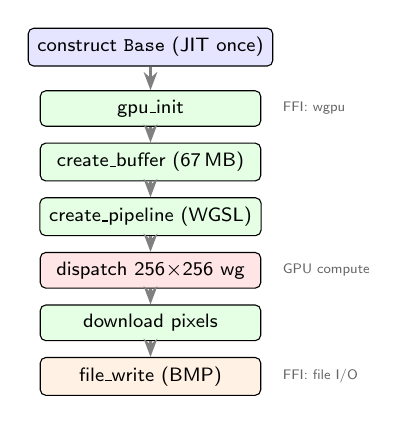
\begin{tikzpicture}[
    >=Stealth,
    step/.style={draw, rounded corners=2pt, minimum height=0.45cm,
                 font=\scriptsize\sffamily, fill=#1, text=black,
                 minimum width=2.8cm, align=center},
    step/.default=gray!8,
    arr/.style={->, thick, color=black!50},
    lbl/.style={font=\tiny\sffamily, text=black!60},
  ]
  \node[step=blue!10] (jit) {construct \texttt{Base} (JIT once)};
  \node[step=green!10, below=0.3 of jit] (init) {gpu\_init};
  \node[step=green!10, below=0.2 of init] (buf) {create\_buffer (67\,MB)};
  \node[step=green!10, below=0.2 of buf] (pipe) {create\_pipeline (WGSL)};
  \node[step=red!10, below=0.2 of pipe] (disp) {dispatch 256$\times$256 wg};
  \node[step=green!10, below=0.2 of disp] (dl) {download pixels};
  \node[step=orange!10, below=0.2 of dl] (wr) {file\_write (BMP)};

  \draw[arr] (jit) -- (init);
  \draw[arr] (init) -- (buf);
  \draw[arr] (buf) -- (pipe);
  \draw[arr] (pipe) -- (disp);
  \draw[arr] (disp) -- (dl);
  \draw[arr] (dl) -- (wr);

  % annotations
  \node[lbl, right=0.15 of init] {FFI: wgpu};
  \node[lbl, right=0.15 of disp] {GPU compute};
  \node[lbl, right=0.15 of wr] {FFI: file I/O};
\end{tikzpicture}
\caption{Path tracer execution: one CLIF function orchestrates the GPU
through FFI calls. Total: ${\sim}$735\,ms.}
\label{fig:raytrace}
\end{figure}

The JIT-compiled native code calls \texttt{cl\_gpu\_init} to initialize
a wgpu~\cite{wgpu} context handle, creates a buffer and pipeline, dispatches $256 \times 256$
workgroups (each covering a $16 \times 16$ pixel tile), downloads the
result into the pixel region of shared memory, and writes the BMP file.
The entire GPU lifecycle---from shader compilation to file output---is
driven by a single Cranelift function that Lean generated and type-checked.

\subsection{What Lean Prevents}

Without dependent types, common errors in this pipeline include:
writing the shader string past its allocated region, using the wrong
pixel buffer offset in the download call, or sizing the BMP header
inconsistently with the pixel format. In Base, the Lean type system can
rule out these classes of mistakes at build time: \texttt{shaderOff} is
a typed field handle whose offset is computed by the layout builder, and
using it with an incompatible size is a type error. In the generated
path-tracer artifact, those checks eliminate the need for corresponding
run-time offset validation in the engine.

% ===================================================================
\section{Build Pipeline}
\label{sec:build}

Figure~\ref{fig:buildpipeline} shows how a Lean source becomes an
executable.

\begin{figure}[H]
\centering
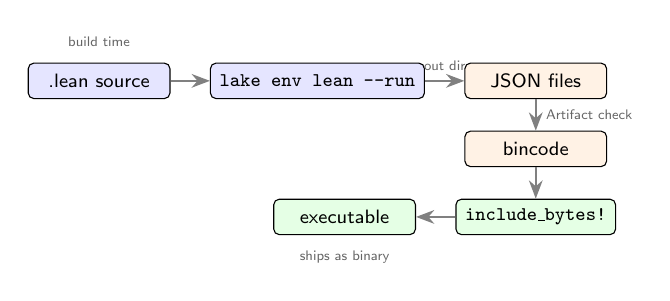
\begin{tikzpicture}[
    >=Stealth,
    box/.style={draw, rounded corners=2pt, minimum height=0.45cm,
                font=\scriptsize\sffamily, fill=#1, text=black,
                minimum width=1.8cm},
    box/.default=gray!8,
    arr/.style={->, thick, color=black!50},
    lbl/.style={font=\tiny\sffamily, text=black!60},
  ]
  \node[box=blue!10] (lean) {.lean source};
  \node[box=blue!10, right=0.5 of lean] (lake) {\texttt{lake env lean {-}{-}run}};
  \node[box=orange!10, right=0.5 of lake] (json) {JSON files};
  \node[box=orange!10, below=0.4 of json] (bin) {bincode};
  \node[box=green!10, below=0.4 of bin] (inc) {\texttt{include\_bytes!}};
  \node[box=green!10, left=0.5 of inc] (exe) {executable};

  \draw[arr] (lean) -- (lake);
  \draw[arr] (lake) -- node[lbl, above] {out dir} (json);
  \draw[arr] (json) -- node[lbl, right] {Artifact check} (bin);
  \draw[arr] (bin) -- (inc);
  \draw[arr] (inc) -- (exe);

  % time labels
  \node[lbl, above=0.08 of lean] {build time};
  \node[lbl, below=0.08 of exe] {ships as binary};
\end{tikzpicture}
\caption{Build pipeline: Lean runs at \texttt{cargo build} time via
\texttt{build.rs}. The data artifact is baked into the Rust binary.}
\label{fig:buildpipeline}
\end{figure}

\texttt{build.rs} first invokes \texttt{lake build} for the Lean module,
then runs \texttt{lake env lean --run <file> <out-dir>}. The Lean program
writes one JSON file per artifact into that output directory. The build
script validates each file against the Rust \texttt{Artifact} type via
\texttt{serde\_json}, re-serializes it to bincode, and writes the result
to \texttt{\$OUT\_DIR}. The Rust binary includes this blob via
\texttt{include\_bytes!} and deserializes it with
\texttt{Artifact::from\_bytes} at startup.

% ===================================================================
\section{Evaluation}
\label{sec:eval}

All benchmarks were run on the same machine: AMD Ryzen 5 5500
(6 cores / 12 threads), NVIDIA RTX 3060 (12\,GB), 32\,GB DDR4, Linux 6.14.
Reported times are medians of 10 rounds from the current harness, and each
row is checked for correctness against a reference implementation. The full
suite is invoked by \texttt{./benchmarks/run.sh}, which builds the Python
extension and Python-generated artifacts first, then delegates the Rust
suite to \texttt{cargo run --release -p benchmarks}. The two suites report
different comparisons: the Python suite compares Python libraries with
PyBase, while the Rust suite compares native Rust, Burn/Rayon where
applicable, and Base.

\subsection{CPU}

\begin{table}[t]
\centering\small
\caption{Python-facing benchmarks. The Python column is Python, NumPy,
Pandas, or PyTorch depending on the row; PyBase is the same Base engine
called through the Python extension.}
\label{tab:py}
\begin{tabular}{@{}lrr@{}}
\toprule
 & \textbf{Python} & \textbf{PyBase} \\
\midrule
CSV 1M        & 496.3\,ms & 26.4\,ms \\
JSON 500K     & 312.8\,ms & 9.44\,ms \\
Regex 1M      & 83.1\,ms  & 4.83\,ms \\
StrSearch 1M  & 3.73\,ms  & 1.51\,ms \\
WordCnt 1M    & 110.2\,ms & 37.4\,ms \\
VecAdd 50M    & 43.5\,ms  & 12.9\,ms \\
Pandas RevAgg 10M & 86.8\,ms & 7.88\,ms \\
RMSNorm 4096  & 0.059\,ms & 0.012\,ms \\
\bottomrule
\end{tabular}
\end{table}

\begin{table}[t]
\centering\small
\caption{Rust CPU file/string benchmarks from the current harness.}
\label{tab:cpu}
\begin{tabular}{@{}lrr@{}}
\toprule
 & \textbf{Rust} & \textbf{Base} \\
\midrule
CSV 10K      & 0.3\,ms   & 1.1\,ms \\
CSV 1M       & 57.6\,ms  & 27.7\,ms \\
CSV 5M       & 310.5\,ms & 141.4\,ms \\
JSON 1K      & 0.0\,ms   & 0.8\,ms \\
JSON 500K    & 15.9\,ms  & 9.7\,ms \\
Regex 10K    & 0.1\,ms   & 0.9\,ms \\
Regex 1M     & 6.7\,ms   & 4.2\,ms \\
StrSearch 1M & 2.2\,ms   & 1.3\,ms \\
WordCnt 1M   & 32.9\,ms  & 37.1\,ms \\
\bottomrule
\end{tabular}
\end{table}

\begin{table}[t]
\centering\small
\caption{Numerical compute (4$\times$-unrolled SIMD in Base).}
\label{tab:num}
\begin{tabular}{@{}lrrr@{}}
\toprule
 & \textbf{Rust} & \textbf{Burn} & \textbf{Base} \\
\midrule
MatMul 128   & 0.2\,ms  & 0.1\,ms   & 0.2\,ms \\
MatMul 512   & 12.0\,ms & 1.1\,ms   & 7.7\,ms \\
MatMul 1024  & 98.9\,ms & 8.1\,ms   & 59.0\,ms \\
VecAdd 1M    & 0.7\,ms  & 0.2\,ms   & 0.1\,ms \\
VecAdd 10M   & 7.2\,ms  & 25.4\,ms  & 2.4\,ms \\
VecAdd 50M   & 36.0\,ms & 117.3\,ms & 12.6\,ms \\
Sum 1M       & 0.7\,ms  & 0.1\,ms   & 0.1\,ms \\
Sum 10M      & 7.1\,ms  & 1.8\,ms   & 1.5\,ms \\
Sum 100M     & 71.4\,ms & 18.5\,ms  & 16.3\,ms \\
\bottomrule
\end{tabular}
\end{table}

On larger file and string-processing workloads, Base is competitive with
and often faster than the current Rust baselines: CSV~5M runs in
141.4\,ms vs.\ 310.5\,ms, JSON~500K in 9.7\,ms vs.\ 15.9\,ms,
Regex~1M in 4.2\,ms vs.\ 6.7\,ms, and StrSearch~1M in 1.3\,ms vs.\
2.2\,ms. Small inputs show the fixed cost of entering the engine and
calling FFI. For workloads such as CSV and Regex, the generated CLIF uses
explicit SIMD instructions such as
\texttt{splat.i8x16}, \texttt{icmp}, and \texttt{vhigh\_bits} rather
than relying on auto-vectorization.

On numerical CPU workloads, Base about matches Rust overall and is
substantially faster than Burn on simple element-wise operations:
VecAdd~10M runs in 2.4\,ms vs.\ 7.2\,ms for Rust and 25.4\,ms for Burn,
and Sum~100M runs in 16.3\,ms vs.\ 71.4\,ms and 18.5\,ms respectively.
Burn still exceeds Base on matmul because it routes to specialized
backend kernels. WordCount is the notable exception on the file-processing side:
at 1M words Base is slower than Rust (37.1\,ms vs.\ 32.9\,ms),
most plausibly because Base goes through external \texttt{ht\_*} FFI
calls that Cranelift cannot inline, whereas LLVM can optimize the Rust
\texttt{HashMap} path more aggressively.

\subsection{GPU, CUDA, and Stress Tests}

\begin{table}[t]
\centering\small
\caption{GPU benchmarks (one-shot: upload + compute + download).}
\label{tab:gpu}
\begin{tabular}{@{}lrr@{}}
\toprule
 & \textbf{Burn (wgpu)} & \textbf{Base} \\
\midrule
VecAdd 256K  & 4.2\,ms & 0.7\,ms \\
VecAdd 500K  & 3.9\,ms & 1.2\,ms \\
MatMul 256   & 3.0\,ms & 0.4\,ms \\
MatMul 512   & 3.9\,ms & 1.2\,ms \\
Reduce 256K  & 3.0\,ms & 0.4\,ms \\
Reduce 512K  & 3.5\,ms & 0.5\,ms \\
Reduce 896K  & 4.1\,ms & 0.8\,ms \\
\bottomrule
\end{tabular}
\end{table}

\begin{table}[t]
\centering\small
\caption{GPU iterative (data stays on device).}
\label{tab:gpuiter}
\begin{tabular}{@{}lrrr@{}}
\toprule
 & \textbf{Raw wgpu} & \textbf{Burn} & \textbf{Base} \\
\midrule
$1\times$ 1M     & 3.9\,ms  & 4.4\,ms  & 1.7\,ms \\
$10\times$ 1M    & 4.0\,ms  & 5.0\,ms  & 2.2\,ms \\
$100\times$ 1M   & 8.5\,ms  & 7.0\,ms  & 6.7\,ms \\
$500\times$ 1M   & 25.8\,ms & 22.5\,ms & 26.9\,ms \\
$1000\times$ 1M  & 49.4\,ms & 41.3\,ms & 49.4\,ms \\
\bottomrule
\end{tabular}
\end{table}

\begin{table}[!t]
\centering\small
\caption{CUDA (direct PTX, no compile-time toolkit).}
\label{tab:cuda}
\begin{tabular}{@{}lrr@{}}
\toprule
 & \textbf{Burn (cuda)} & \textbf{Base} \\
\midrule
SAXPY 262K  & 0.5\,ms & 0.5\,ms \\
SAXPY 524K  & 0.9\,ms & 0.8\,ms \\
SAXPY 1M    & 1.8\,ms & 1.7\,ms \\
\bottomrule
\end{tabular}
\end{table}

On one-shot GPU workloads, Base is consistently faster than Burn's
\texttt{wgpu} backend: VecAdd~256K runs in 0.7\,ms vs.\ 4.2\,ms,
MatMul~512 in 1.2\,ms vs.\ 3.9\,ms, and Reduce~896K in 0.8\,ms vs.\ 4.1\,ms.
Because both implementations use \texttt{wgpu} on the same hardware,
this is primarily a difference in host-side runtime overhead rather than
a different GPU path.

The iterative GPU-resident benchmark is more balanced. Base wins at
$1\times$ and $10\times$ passes (1.7\,ms and 2.2\,ms), remains close at
$100\times$, and by $500\times$--$1000\times$ passes Burn and raw wgpu
catch up or pull ahead. That is consistent with a workload that becomes
dominated by repeated kernel execution rather than orchestration. CUDA is
also close: Base runs SAXPY~1M in 1.7\,ms versus 1.8\,ms for Burn(cuda).

\begin{table}[!t]
\centering\small
\caption{Parallel histogram.}
\label{tab:par}
\begin{tabular}{@{}lrrr@{}}
\toprule
 & \textbf{Rust} & \textbf{Rayon} & \textbf{Base} \\
\midrule
Hist 1M $w$=1   & 1.1\,ms  & 1.0\,ms  & 1.6\,ms \\
Hist 1M $w$=4   & 0.8\,ms  & 0.9\,ms  & 1.4\,ms \\
Hist 10M $w$=1  & 10.8\,ms & 11.5\,ms & 10.8\,ms \\
Hist 10M $w$=4  & 8.6\,ms  & 8.4\,ms  & 7.9\,ms \\
\bottomrule
\end{tabular}
\end{table}

Table~\ref{tab:par} shows an additional CPU-side stress test. Base is
close on parallel histogramming.

% ===================================================================
\section{Conclusion}
\label{sec:conclusion}

Base separates dependent-type verification (Lean~4, build time) from native
execution (Rust engine, Cranelift JIT, run time) through a serializable
\texttt{Artifact}. No type checker runs at run time. On the evaluated
workloads, it is competitive with idiomatic Rust and native GPU frameworks.

The artifact is emitted as JSON at build time and embedded as bincode at
run time, so the model extends naturally to board-level programming. Today
the engine dispatches to CPU,
and exposes FFI primitives for wgpu, CUDA, networking, file I/O, LMDB,
and threading. Each device keeps its awkward ISA; Lean verifies cross-device
constraints at build time, and the engine orchestrates at run time.

Any Lean code that produces a valid \texttt{Artifact} is a legitimate front end.
The monadic DSLs presented here are one choice; users are free to build
higher-level representations---algebraic IRs, domain-specific abstractions,
or full compiler pipelines---and have dependent types flow through to the
final algorithm emission. Layout errors, offset mismatches, and
device-compatibility constraints can all be caught interactively as
programmers construct objects, making the value of dependent types
immediately visible rather than deferred to a separate verification step.

Base targets CPU and GPU backends at the driver-API level---Cranelift for
native code, the CUDA driver API for PTX, and wgpu for portable GPU
compute---and exposes them to Lean as FFI primitives. This means the
optimization and orchestration logic that would otherwise live in a C++
compiler stack can instead be written in Lean, where a strong type system
and proof assistant make it simpler to write correct transformations.

% ===================================================================
\begin{thebibliography}{9}

\bibitem{lean4}
L.~de Moura and S.~Ullrich,
``The Lean~4 theorem prover and programming language,''
in \emph{Proc.\ CADE-28}, 2021.

\bibitem{cranelift}
Bytecode Alliance,
``Cranelift code generator,''
\url{https://cranelift.dev}, 2024.

\bibitem{llvm}
C.~Lattner and V.~Adve,
``LLVM: A compilation framework for lifelong program analysis and
transformation,''
in \emph{Proc.\ CGO}, 2004.

\bibitem{wgpu}
gfx-rs contributors,
``wgpu: Safe and portable GPU abstraction,''
\url{https://wgpu.rs}, 2024.

\bibitem{lmdb}
H.~Chu,
``LMDB: Lightning memory-mapped database,''
\url{http://www.lmdb.tech/doc/}, 2011.

\bibitem{burn}
Burn contributors,
``Burn: A flexible and comprehensive deep learning framework in Rust,''
\url{https://burn.dev}, 2024.

\end{thebibliography}

\end{document}
